%%%% Better Poster latex template example v1.0 (2019/04/04)
%%%% GNU General Public License v3.0
%%%% Rafael Bailo
%%%% https://github.com/rafaelbailo/betterposter-latex-template
%%%% 
%%%% Original design from Mike Morrison
%%%% https://twitter.com/mikemorrison

\documentclass[a0paper,fleqn]{src/betterposter}

\begin{document}	
\betterposter{
%%%%%%%% MAIN COLUMN

\maincolumn{
%%%% Main space

\vspace{-3cm}
\textbf{Metapackage structure}\\
\fontsize{75}{77}\selectfont % Set the font size to 12pt with a baseline skip of 14pt

Required and extra dependencies groups\\[1.5cm]
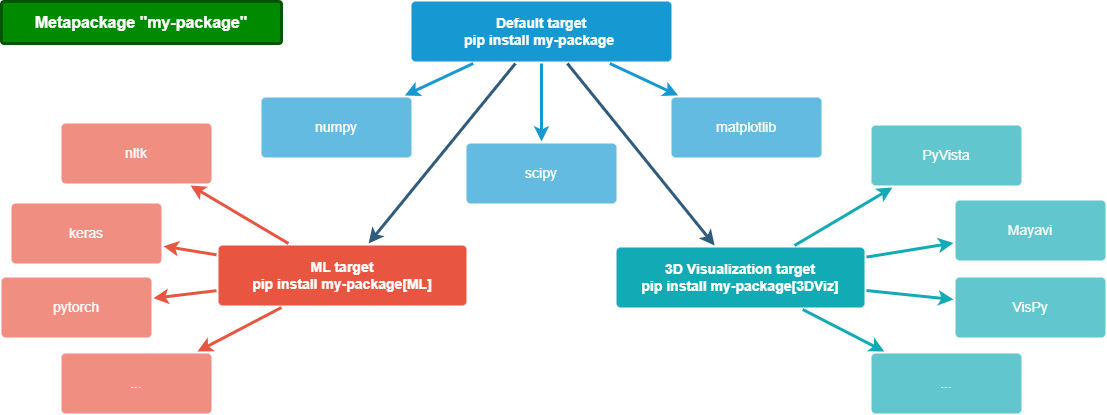
\includegraphics[width=\textwidth]{img/metapackage/deps}\\

Metapackage layout\\[1.5cm]
\hspace{5cm}
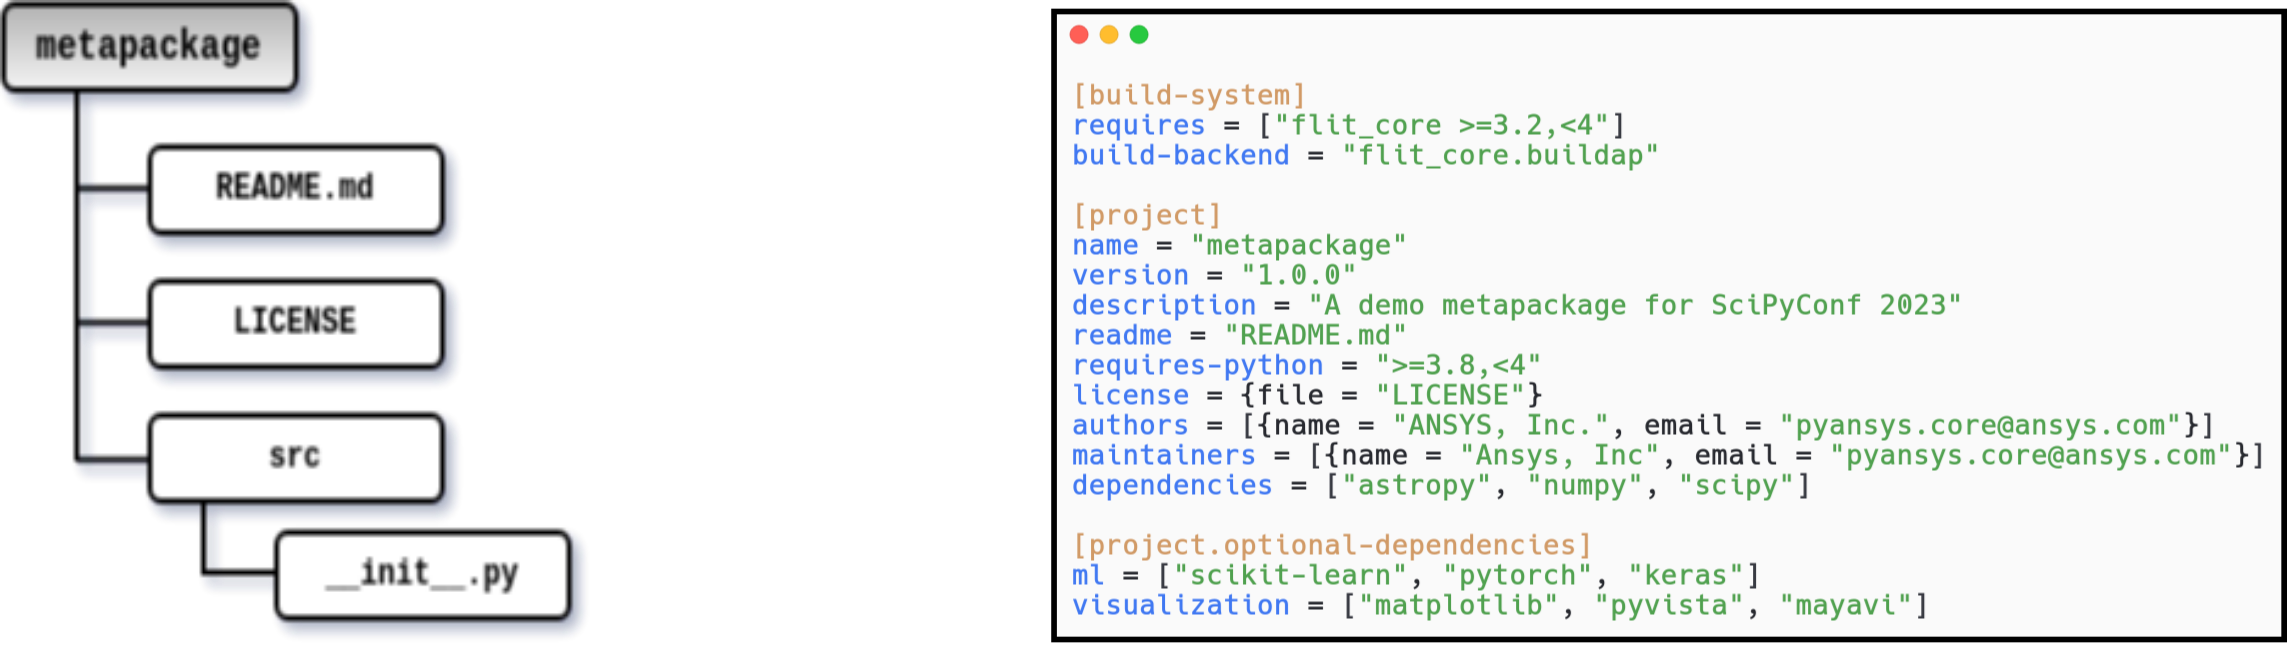
\includegraphics[width=0.98\textwidth]{img/metapackage/layout}\\

\vspace{-15cm}
}{
%%%% Bottom space

%% QR code
\qrcode{img/metapackage/qrcode.png}{img/general/smartphoneBlack}{
\textbf{Want to see an example repository?} \\ \checkmark Visit https:\slash \slash github.com/ansys/pyansys \\ \newline \textbf{Any questions?} \\ \checkmark Don't be shy and start the conversation!

}
% Smartphone icon
% Author: Freepik
% Retrieved from: https://www.flaticon.com/free-icon/smartphone_65680

%% Compact QR code (comment the previous command and uncomment this one to switch)
%\compactqrcode{img/example/qrcode}{
%\textbf{Take a picture} to
%\\download the full paper
%}

}

}{
%%%%%%%% LEFT COLUMN

\title{Python \\metapackages}
\author{Roberto Pastor Muela}
\institution{Ansys}

\section{
\includegraphics[height=\fontcharht\font`\S]{img/general/slash.png} Introduction}
Organizations experience problems when distributing multiple packages. What if you could easily distribute
all your packages in one single package? Python \textit{metapackages} are here to solve your problems!

\section{
\includegraphics[height=\fontcharht\font`\S]{img/general/slash.png} The \textit{metapackage}\\concept}
Python \textit{metapackages} are empty Python libraries that contain only a version attribute.
However, they use a "dependencies" section to declare all libraries that are required for the
installation. This trick can be used to install all the desired projects of a large community.

\section{
\includegraphics[height=\fontcharht\font`\S]{img/general/slash.png} Example use case}
Say you have a Python metapackage called \textit{my-package}. By installing it, users get your
defined dependencies and also have access to additional targets you define. See the graph on the main
section of this poster.

\section{
\includegraphics[height=\fontcharht\font`\S]{img/general/slash.png} File structure}
\vspace{-2cm}
\begin{itemize}
    \item The \texttt{src/<my-package>} folder has an \texttt{\_\_init\_\_.py} file that simply contains your metapackage version.
    \item A build system requirements file, \texttt{pyproject.toml}, \texttt{setup.py}), contains with your dependencies and extra targets. Dependency versions can be pinned down. For example, \texttt{numpy==1.21.0}) or flexible (\texttt{numpy}).
\end{itemize}

%% This fills the space between the content and the logo
\vfill

}{
%%%%%%%% RIGHT COLUMN
\section{
\includegraphics[height=\fontcharht\font`\S]{img/general/slash.png} Benefits of using a\\ metapackage}
\vspace{-2cm}
\begin{itemize}
    \item \underline{\textbf{One-stop shop}}: All your Python packages are delivered together and are easily made available to end users.
    \item \underline{\textbf{Dependencies compatibility}}: No incompatibility issues amongst dependencies can occur (when using CI/CD for building the package).
    \item \underline{\textbf{Easier install process}}: Rather than installing each package individually, install all packages with only one installation command.
    \item \underline{\textbf{Multiple targets}}: The metapackage may not only have \textit{required} dependencies, it may also have extra targets (additional dependencies) for other purposes.
    \item \underline{\textbf{Pinned versions}} (optional): Dependency updates sometimes lead to incompatibilities that users are not aware of. By having a metapackage that pins down your dependencies to a certain version, you make sure that for a given version your scripts are compatible with all the dependent libraries. This makes dependency handling much easier for end users.

\end{itemize}
\vfill

%% Institution logo

\includegraphics[width=\textwidth]{img/general/pyansys_dark}\\
The PyAnsys project is a collection of Python packages that enable the use of Ansys products through Python.
\\
\newline
\textbf{Any questions?} \\Contact us at pyansys.core@ansys.com.
\\
\newline

\qrcode{img/general/pyansys_qrcode.png}{img/general/smartphoneBlack}{
\textbf{\huge{See our docs for more\\information on PyAnsys:\\https:\slash \slash docs.pyansys.com }}
}
}
\end{document}
